% In questo file vengono definiti comandi (macro) utili in tutti i documenti

\newcommand{\gruppo}{\textit{Sirius}} % nome gruppo
\newcommand{\progetto}{\textit{Sequenziatore}} % nome progetto
\newcommand{\capitolato}{\href{http://www.math.unipd.it/~tullio/IS-1/2013/Progetto/C4p.pdf}{http://www.math.unipd.it/~tullio/IS-1/2013/Progetto/C4p.pdf}} 

% GLOSSARIO
\newcommand{\lastversionG}{4.0.0}
\newcommand{\Glossario}{\textit{Glossario\_{}v\lastversionG{}.pdf}}
\newcommand{\doctitleG}{Glossario}
\newcommand{\infoG}{\doctitleG\ v\lastversionG}

% NORME DI PROGETTO
\newcommand{\lastversionNDP}{4.0.0}
\newcommand{\NormeDiProgetto}{\textit{NormeDiProgetto\_{}v\lastversionNDP{}.pdf}}
\newcommand{\doctitleNDP}{Norme di progetto}
\newcommand{\infoNDP}{\doctitleNDP\ v\lastversionNDP}

% ANALISI DEI REQUISITI
\newcommand{\lastversionAR}{3.0.0}
\newcommand{\AnalisiDeiRequisiti}{\textit{AnalisiDeiRequisiti\_{}v\lastversionAR{}.pdf}}
\newcommand{\doctitleAR}{Analisi dei requisiti}
\newcommand{\infoAR}{\doctitleAR\ v\lastversionAR}

% Studio di fattibilita
\newcommand{\lastversionSDF}{2.0.0}
\newcommand{\StudioDiFattibilita}{\textit{StudioDiFattibilita\_{}v\lastversionSDF{}.pdf}}
\newcommand{\doctitleSDF}{Studio Di Fattibilità}
\newcommand{\infoSDF}{\doctitleSDF\ v\lastversionSDF}

% Piano di qualifica
\newcommand{\lastversionPDQ}{4.0.0}
\newcommand{\PianoDiQualifica}{\textit{PianoDiQualifica\_{}v\lastversionPDQ{}.pdf}}
\newcommand{\doctitlePDQ}{Piano Di Qualifica}
\newcommand{\infoPDQ}{\doctitlePDQ\ v\lastversionPDQ}

% VERBALE 2014-02-03
\newcommand{\lastversionVb}{2.0.0}
\newcommand{\VerbaleB}{\textit{Verbale2014-02-03\_{}v\lastversionVb{}.pdf}}
\newcommand{\doctitleVb}{Verbale 2014-02-03}
\newcommand{\infoVb}{\doctitleVb\ v\lastversionVb}

% VERBALE 2014-07-20
\newcommand{\lastversionVN}{1.0.0}
\newcommand{\VerbaleN}{\textit{Verbale2014-07-20\_{}v\lastversionVN{}.pdf}}
\newcommand{\doctitleVN}{Verbale 2014-07-20}
\newcommand{\infoVN}{\doctitleVN\ v\lastversionVN}

%Piano di progetto
\newcommand{\lastversionPDP}{4.0.0}
\newcommand{\PianoDiProgetto}{\textit{PianoDiProgetto\_{}v\lastversionPDP{}.pdf}}
\newcommand{\doctitlePDP}{Piano Di Progetto}
\newcommand{\infoPDP}{\doctitlePDP\ v\lastversionPDP}
%Specifica Tecnica
\newcommand{\lastversionST}{3.0.0}
\newcommand{\SpecificaTecnica}{\textit{SpecificaTecnica\_{}v\lastversionST{}.pdf}}
\newcommand{\doctitleST}{Specifica Tecnica}
\newcommand{\infoST}{\doctitleST\ v\lastversionST}
%Definizione di prodotto
\newcommand{\lastversionDP}{2.0.0}
\newcommand{\DefinizioneDiProdotto}{\textit{DefinizioneDiProdotto\_{}v\lastversionDP{}.pdf}}
\newcommand{\doctitleDP}{Definizione Di Prodotto}
\newcommand{\infoDP}{\doctitleDP\ v\lastversionDP}

% MANUALE UTENTE
\newcommand{\lastversionMU}{2.0.0}
\newcommand{\ManualeUtente}{\textit{ManualeUtente\_{}v\lastversionMU{}.pdf}}
\newcommand{\doctitleMU}{Manuale utente}
\newcommand{\infoMU}{\doctitleMU\ v\lastversionMU}

% MANUALE PROCESS OWNER
\newcommand{\lastversionMPO}{2.0.0}
\newcommand{\ManualePO}{\textit{ManualeProcessOwner\_{}v\lastversionMPO{}.pdf}}
\newcommand{\doctitleMPO}{Manuale process owner}
\newcommand{\infoMPO}{\doctitleMPO\ v\lastversionMPO}% macro
\newcommand{\lastversion}{\lastversionMU}%versione del documento
\newcommand{\doctitle}{\doctitleMU}%nome documento
\newcommand{\info}{\doctitle\ v\lastversion}
\documentclass[11pt,a4paper]{article}
\usepackage[a4paper,portrait,top=3.5cm,bottom=3.5cm,left=3cm,right=3cm,bindingoffset=5mm]{geometry}


\usepackage[italian]{babel}
\usepackage{ucs} %unicode sistema gli accenti
\usepackage[utf8x]{inputenc} %unicode sistema gli accenti
\usepackage{fancyhdr}
\usepackage{subfigure} % per figure affiancate
\usepackage{hyperref}
\usepackage{float} % per far bene le figures
\usepackage{indentfirst}
\usepackage{longtable}
\usepackage{color}
\usepackage{colortbl}
\usepackage{rotating}
\usepackage[table]{xcolor}
\usepackage{wrapfig}
\usepackage{array}
\usepackage{eurosym}
\usepackage{graphicx}
\usepackage{breakurl}
\usepackage{lastpage} % total page count
\usepackage{chngpage}
\usepackage{amsfonts}
\usepackage{listings}
\usepackage{bookmark} % custom bookmarks

%\graphicspath{{./Pics}} % cartella di salvataggio immagini

% Per l'indice analitico
%\usepackage{makeidx}
%\makeindex

%pagestyle{fancy}
%\renewcommand{\chaptermark}[1]{\markboth{\thechapter.\ #1}{}}
%\renewcommand{\sectionmark}[1]{\markright{\thesection.\ \ #1}{}}
%\fancyhead{}
%comandi dell header
%\fancyhead[EL]{\slshape \leftmark}
%\fancyhead[OR]{\slshape \rightmark}
%\fancyfoot[EC,OC]{\slshape \thepage}

\pagestyle{fancy}
%\newcommand{\license}{\href{http://creativecommons.org/licenses/by/3.0/}{Some rights reserved}}
\newcommand{\groupname}{Sirius - Sequenziatore}

\newcommand{\subscript}[1]{\raisebox{-0.6ex}{\scriptsize #1}}
%\newcommand{\subscript}[1]{\ensuremath{_{\textrm{#1}}}}
%\renewcommand{\sectionmark}[1]{\markright{\thesection.\ #1}}
%\lhead{\nouppercase{\rightmark}}
%\rhead{\nouppercase{\leftmark}}
%\renewcommand{\chaptermark}[1]{\markboth{\thechapter.\ #1}{}}


\fancypagestyle{plain}{%
	\chead{}
	\lfoot{\info}
	\cfoot{}
	\rfoot{\thepage\ / \pageref{LastPage}}
	\renewcommand{\headrulewidth}{0.3pt}
	\renewcommand{\footrulewidth}{0.3pt}
}
	\lhead{\setlength{\unitlength}{1mm}
        \begin{picture}(0,0)
                \put(5,0){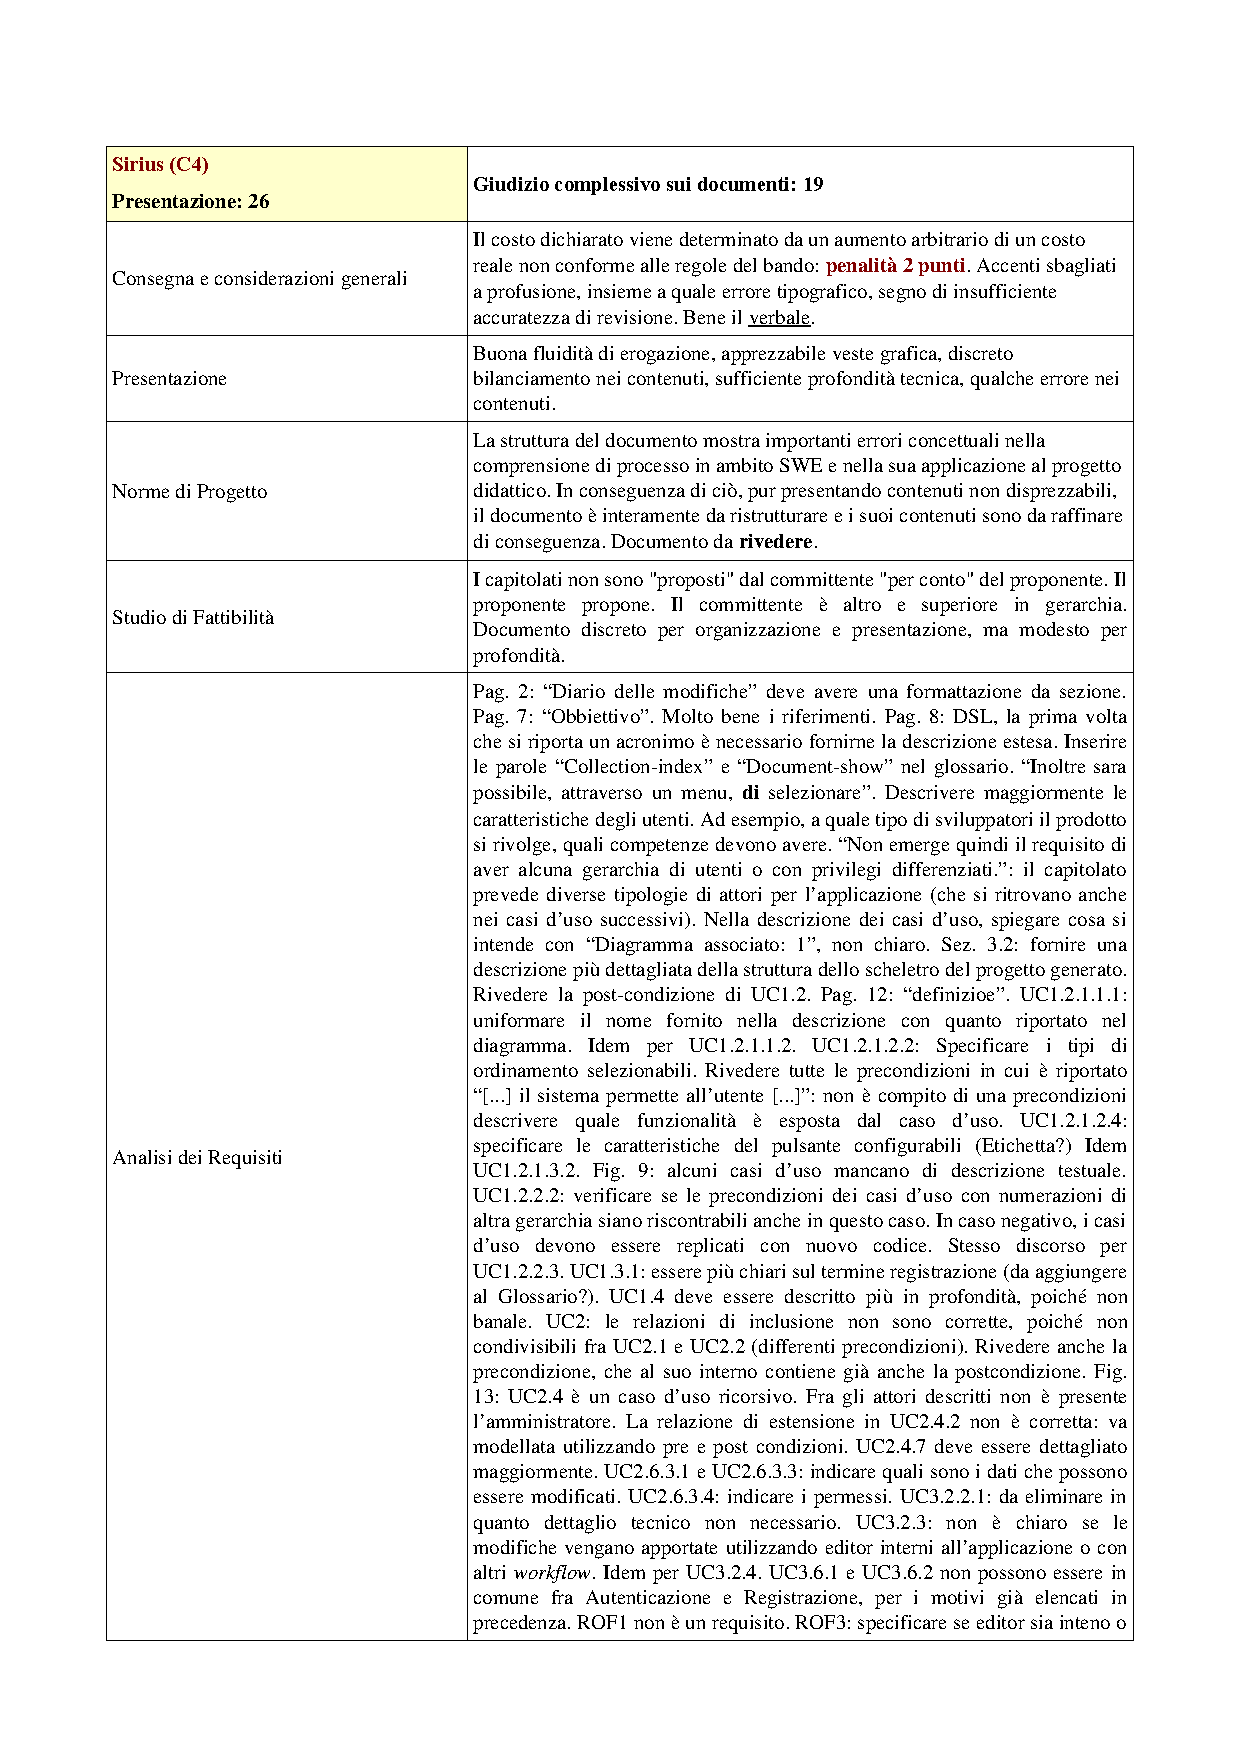
\includegraphics[scale=0.001]{img/Sirius.png}}
        \end{picture}}
	\rhead{\groupname}
	\chead{}
	\lfoot{\info}
	\cfoot{}
%	\rfoot{\thepage}
	\rfoot{\thepage\ / \pageref{LastPage}}
	\renewcommand{\headrulewidth}{0.3pt}
	\renewcommand{\footrulewidth}{0.3pt}
\linespread{1.2}	% valore interlinea


\fancypagestyle{romano}{
	\lhead{\setlength{\unitlength}{1mm}
        \begin{picture}(0,0)
                \put(5,0){
\includegraphics[scale=0.03]{../modello/img/sirius.png}}
        \end{picture}}
	\chead{}
	\rhead{\groupname}
	\lfoot{\info}
	\cfoot{}
	\rfoot{\thepage}
	\renewcommand{\headrulewidth}{0.3pt}
	\renewcommand{\footrulewidth}{0.3pt}
}



\hypersetup{
    colorlinks=true,linkcolor=[rgb]{0.11,0.55,0.83
    },          % colore link interni
    urlcolor=cyan           %colore link esterni
}
\definecolor{err}{rgb}{0.9,0.1,0.1}
\definecolor{rt}{rgb}{0.1,0.6,0.8}
\definecolor{grey}{rgb}{0.4,0.3,0.4}
\definecolor{mycolor}{rgb}{0.67,1,0.18}

\bibliographystyle{plain_ita}%bibliografia stile italiano

\pagenumbering{Roman}
\setlength\parindent{0pt} % sempre senza indentatura
% fine layout% layout

\makeatletter
\renewcommand*{\BreakableSlash}{%
  \leavevmode
  \prw@zbreak
  %
  \discretionary{-}{}{}%
  \prw@zbreak
}

\tolerance 1414
\hbadness 1414
\emergencystretch 1.5em
\hfuzz 0.3pt
\widowpenalty=10000
\vfuzz \hfuzz
\raggedbottom


\begin{document}

% Prima pagina di opgni documento
\begin{titlepage}
 \begin{center}
     
\includegraphics[width=11cm]{../modello/img/sirius}\\
     \vspace{1em}
     {\LARGE \textsc{Sirius}}\\
     \vspace{2em} \hrule \vspace{2em}
     {\Large \textsc{Sequenziatore}}\\
     \vspace{8em}
     {\LARGE \LARGE \LARGE \textbf{\doctitle}}\\
     \vspace{2em}
     {\LARGE \LARGE \LARGE \textbf{Versione \lastversion }}\\
     \vspace{4em}
 \end{center}


\vskip 1.8cm
\begin{center}
\textit{Ingegneria Del Software AA 2013-2014}
\end{center}

\end{titlepage}


%pagina del titolo
\thispagestyle{romano}
\noindent\begin{Large}\textbf{Informazioni documento}\end{Large}\\
\begin{center}
\begin{tabular}{ll}
\hline\\
Titolo documento: & Analisi dei requisiti\\
Data creazione: & 1 Febbraio 2014\\
Versione attuale: & \lastversion\\
Utilizzo: & Esterno\\
Nome file:& \AnalisiDeiRequisiti{}\\
Redazione: & Botter Marco\\
& Giachin Vanni\\
& Marcomin Gabriele\\
Verifica: & Seresin Davide\\
Approvazione: & Quaglio Davide\\
Distribuito da:& Sirius\\
Destinato a: & Prof. Vardanega Tullio\\
			 & Prof. Cardin Riccardo\\
			 & Zucchetti S.p.A.
\end{tabular}
\end{center}
\vskip 1.5cm
%\noindent {\begin{LARGE}\textbf{Sommario}\end{LARGE}}\\
\noindent\begin{Large}\textbf{Sommario}\end{Large}\\

\noindent Risultato dello studio di fattibilità della ditta Sirius per il capitolato C04 Seq\\
\newpage
\pagestyle{romano}
\noindent\begin{Large}\textbf{Diario delle modifiche}\end{Large}\\
\\
%Inserire in testa ogni nuova versione\\
\begin{small}
\begin{tabular}{|c|p{1.8cm}|p{2.8cm}|p{2.8cm}|p{3.5cm}|}
\hline
Versione & Data & Autore & Ruolo & Descrizione \\
\hline
\hline
1.0.0 & 2014-03-05 & 
\textit{Quaglio Davide} &
\textit{Responsabile} &  Approvazione del documento\\
\hline
0.1.0 & 2014-02-13 & 
\textit{Botter Marco} &
\textit{Verificatore} &  Verifica del documento\\
\hline
0.0.2 & 2014-02-11 & 
\textit{Seresin Davide} &
\textit{Analista} &  Aggiunte e modifiche\\
\hline
0.0.1 & 2014-02-09 & 
\textit{Santangelo Davide} &
\textit{Analista} &  Creato lo scheletro del documento\\
\hline
\end{tabular}\\
\end{small}


\newpage
\pagestyle{romano}

\tableofcontents %sommario
\pagestyle{romano}



\newpage
\pagestyle{plain}
\listoftables
\listoffigures
\pagenumbering{arabic}%numeri di pagina  arabi

\section{Introduzione}

\subsection{Scopo del documento}
Il documento definisce le norme, convenzioni e formalismi  che ciascun membro del gruppo \gruppo{} deve adottare durante l'intera produzione del software \progetto{}.
In particolare tali norme regolamentano i seguenti aspetti:

\begin{itemize}
\item Organizzazione tra i membri del gruppo;
\item Stili e convenzioni nella redazione dei documenti;
\item Metodi operativi e convenzioni nelle fasi di progetto;
\item Ambiente di lavoro.
\end{itemize}

\subsection{Glossario}
Al fine di facilitare la comprensione dei documenti, i termini tecnici, di dominio e gli acronimi, sono definiti in dettaglio nel documento GLOSSARIO.\\
Tali termini sono contrassegnati dal simbolo \ped{$\vert$G$\vert$} che li segue.
%\section{Descrizione generale}
\subsection{Prospettive del prodotto}
Il prodotto si pone,in primo luogo, di realizzare dei processi definiti da una serie
di passi che devono essere eseguiti in sequenza, sia con l' obbligo di terminare i passi precedenti
per accedere al passo successivo, sia con la possibilità di eseguire i passi senza
un ordine predefinito.\\
Oltre a questo il sistema dovrà essere capace di gestire l' esecuzione dei vari passi da parte di
utenti dotati di dispositivo mobili di tipo smartphone, ricevendo da questi ultimi la
richiesta di completamento di un passo; esso sarà accompagnato da vari dati come foto, la posizione geografica e il tempo di completamento. Oltre alla esecuzione, il sistema dovrà essere in grado di poter determinare se il passo è stato eseguito con successo o meno, in base ai dati forniti. 
\subsection{Funzionalità del prodotto}
\subsection{Caratteristiche degli utenti}
\subsection{Vincoli generali}


\section{Istruzioni per l'uso}
\label{istruzioni}

Il presente capitolo offre una visione e una guida al corretto utilizzo delle principali funzionalità disponibili all'utente \textit{process owner\ped{G}}.\\
Sono presenti le seguenti sezioni:

\begin{itemize}
\item  \hyperref[autenticazione]{Autenticazione};
\item  \hyperref[home]{Navigazione nella pagina principale};
\item  \hyperref[creazione]{Creazione di un processo};
\item  \hyperref[controllo]{Controllo e approvazione di un passo};
\item  \hyperref[gestione]{Gestione di un processo};
\item  \hyperref[logout]{Chiusura della sessione}.
\end{itemize}

\pagebreak

\subsection{Autenticazione}
\label{autenticazione}

In figura \hyperref[fig:Flogin]{figura \ref{fig:Flogin}}, è rappresentata la schermata iniziale del prodotto \progetto{}, in cui viene richiesto l'inserimento dello \textit{username} e della \textit{password} dell'utente.

\begin{figure}[H] \centering 
\frame{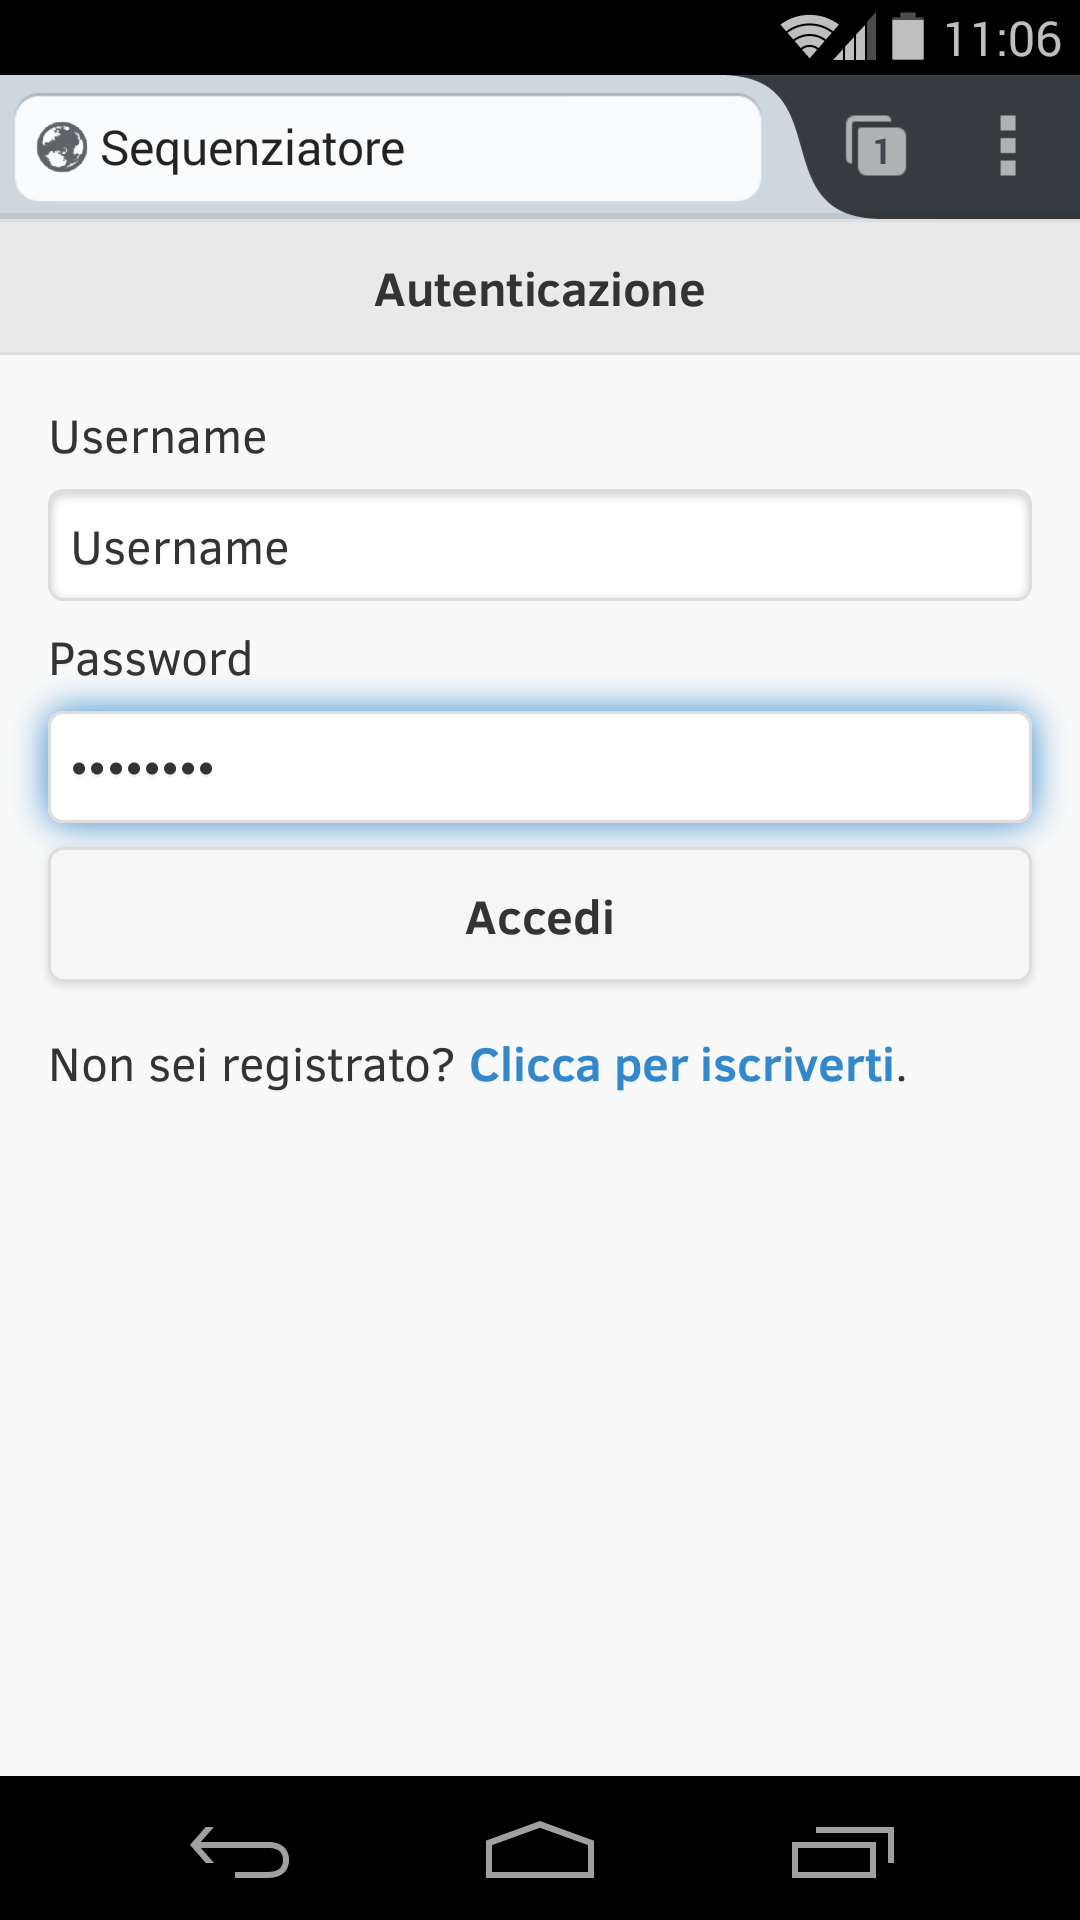
\includegraphics[width=0.5\textwidth]
{./screen/Login.png}} \caption{Schermata di autenticazione}
\label{fig:Flogin}
\end{figure}

Le credenziali di \textit{default} fornite per l'utente \textit{process owner}, sono le seguenti:
\begin{itemize}
\item \textbf{username:} ProcessOwner
\item \textbf{password:} siriusPO
\end{itemize}
Successivamente all'inserimento delle credenziali, è sufficiente selezionare il pulsante ``Accedi'', per accedere alle funzionalità dell'applicazione.

\subsubsection*{Possibili errori:}
\begin{itemize}
\item \hyperref[e1]{E1}: \textit{javascript\ped{G}} disabilitato;
\item \hyperref[e2]{E2}: credenziali non corrette;
\item \hyperref[e3]{E3}: errore di connessione al \textit{server\ped{G}}.
\end{itemize}


\subsection{Navigazione nella pagina principale}
\label{home}
In figura \hyperref[fig:Fhome]{figura \ref{fig:Fhome}}, è rappresentata la schermata della \textit{homepage} del progetto \progetto{}, accessibile dopo aver effettuato l'autenticazione, che consente di scegliere una delle funzionalità di base disponibili al \textit{process owner\ped{G}}.

\begin{figure}[H] \centering 
\frame{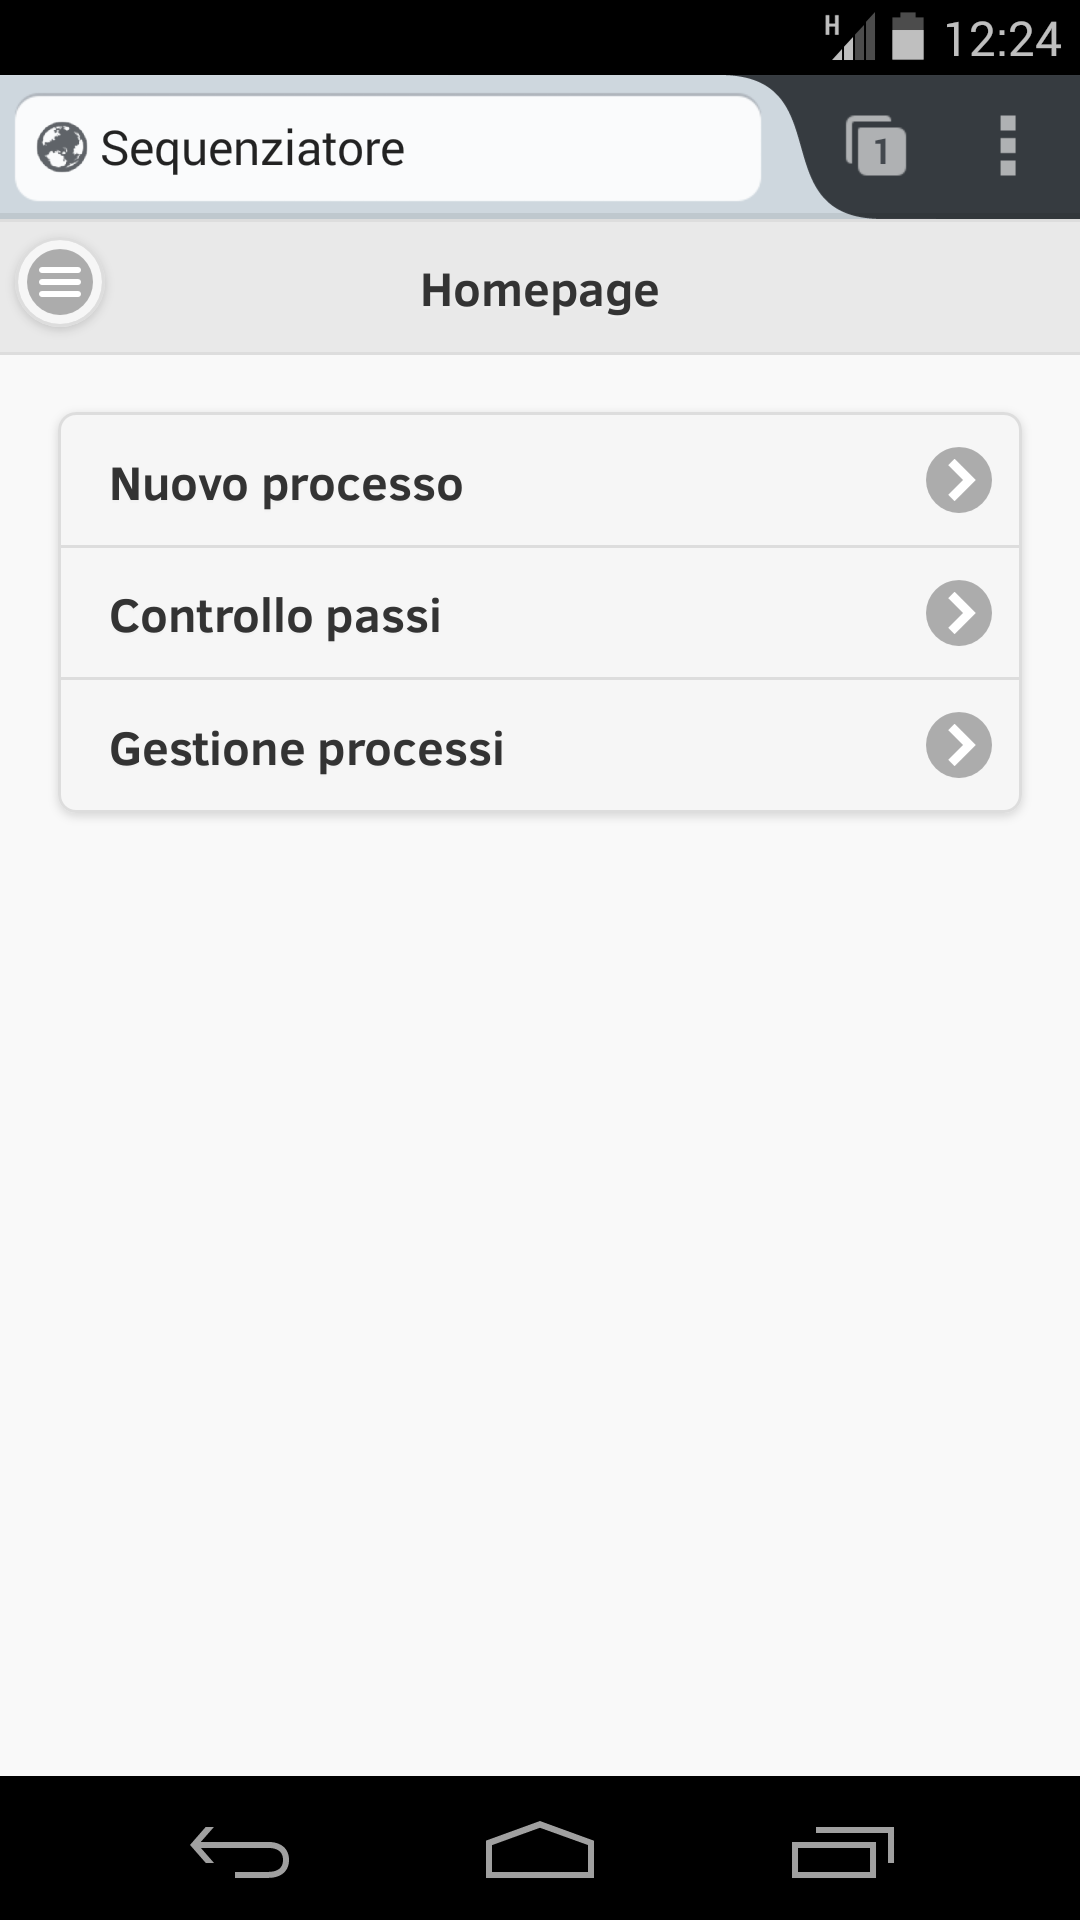
\includegraphics[width=0.5\textwidth]
{./screen/Home.png}} \caption{Homepage}
\label{fig:Fhome}
\end{figure}

È possibile selezionare uno dei seguenti pulsanti per iniziare la gestione delle rispettive funzionalità:
\begin{itemize}
\item  \hyperref[creazione]{Nuovo processo};
\item  \hyperref[controllo]{Controllo passi};
\item  \hyperref[gestione]{Gestione processi}.
\end{itemize}

Selezionando il pulsante in alto a sinistra, è possibile aprire il pannello laterale in cui è consentita la \hyperref[logout]{chiusura della sessione}.

\subsubsection*{Possibili errori:}
\begin{itemize}
\item \hyperref[e1]{E1}: \textit{javascript\ped{G}} disabilitato.
\end{itemize}

\subsection{Creazione di un processo}
\label{creazione}

\subsubsection{Definizione di un processo}
\label{definizione}
\iffalse
In figura \hyperref[fig:Fnewprocess]{figura \ref{fig:Fnewprocess}}, è rappresentata la schermata di scelta di un creazione di un processo, accessibile dopo aver effettuato l'autenticazione.

\begin{figure}[H] \centering 
\frame{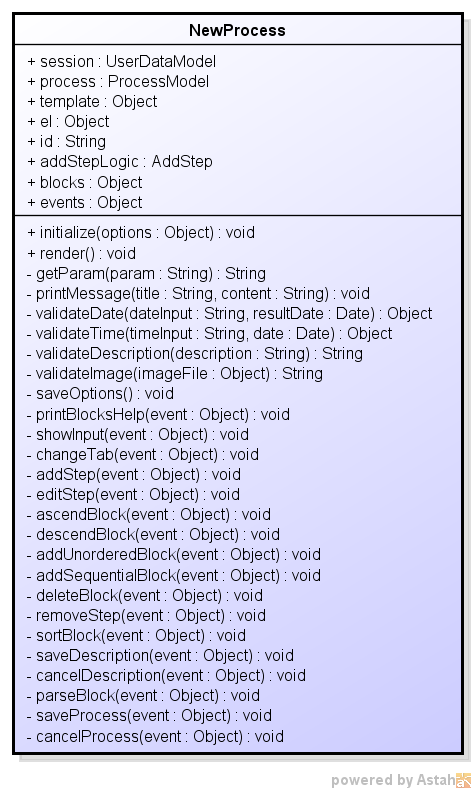
\includegraphics[width=0.5\textwidth]
{./screen/NewProcess.png}} \caption{Creazione di un processo}
\label{fig:Fcheckstep}
\end{figure}
\fi

In questa pagina è possibile definire un nuovo processo.
Viene richiesto l'inserimento dei seguenti dati:
\begin{itemize}
\item \textbf{Nome:} nome del processo, utile alla sua identificazione;
\item \textbf{Descrizione:} breve descrizione, che sarà utile agli utenti per capire lo scopo del processo;
\item \textbf{Criteri di completamento (facoltativi):} 
\begin{itemize}
\item \textbf{Data di terminazione:} Data e orario in cui il processo si concluderà in automatico;
\item \textbf{Numero massimo di completamenti:} Numero di completamenti del processo il quale, una volta raggiunto, comporta la conclusione automatica del processo.
\end{itemize}
\end{itemize}

Nella pagina sono presenti i seguenti pulsanti:
\begin{itemize}
\item \textbf{Aggiungi passo:} \hyperref[addstep]{aggiunge un passo} al processo in definizione;
\item \textbf{Salva processo:} salva il processo in definizione. Se l'operazione si conclude senza errori, il processo diventa disponibile all'iscrizione da parte degli utenti;
\item \textbf{Annulla:} ritorna alla \hyperref[home]{pagina principale}, annullando l'operazione di creazione del processo.
\end{itemize}
Per ogni passo creato sono disponibili inoltre i pulsanti:
\begin{itemize}
\item \textbf{Aggiungi criterio di superamento:} consente di aggiungere un \hyperref[vincoli]{criterio di superamento} al passo;
\item \textbf{Rimuovi passo:} rimuove il passo dal processo in definizione.
\end{itemize}
Infine in altro a sinistra sono presenti i seguenti pulsanti:
\begin{itemize}
\item \textbf{Home:} pulsante che consente di tornare alla \hyperref[home]{pagina principale};
\item \textbf{Opzioni:} apre il pannello laterale in cui è consentita la \hyperref[logout]{chiusura della sessione}.
\end{itemize}

\paragraph*{Possibili errori:}
\begin{itemize}
\item \hyperref[e1]{E1}: \textit{javascript\ped{G}} disabilitato;
\item \hyperref[e3]{E3}: errore di connessione al \textit{server\ped{G}};
\item \hyperref[e4]{E4}: nome processo già utilizzato;
\item \hyperref[e5]{E5}: dato obbligatorio mancante.
\end{itemize}

\subsubsection{Aggiunta di un passo}
\label{addstep}
\iffalse
In figura \hyperref[fig:Faddstep]{figura \ref{fig:Faddstep}}, è rappresentata la schermata di aggiunta di un passo ad un processo in definizione.

\begin{figure}[H] \centering 
\frame{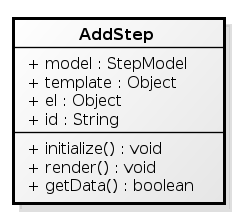
\includegraphics[width=0.5\textwidth]
{./screen/AddStep.png}} \caption{Aggiunta di un passo}
\label{fig:Faddstep}
\end{figure}
\fi

In questa pagina è possibile aggiungere un passo ad un processo in definizione.
Viene richiesto l'inserimento di una breve descrizione, che sarà utile agli utenti per capire lo scopo del passo.

Nella pagina sono presenti i seguenti pulsanti:
\begin{itemize}
\item \textbf{Aggiungi dato:} consente di aggiungere un dato al passo in definizione;
\item \textbf{Salva passo:} aggiunge il passo al processo in creazione;
\item \textbf{Annulla:} ritorna alla \hyperref[newprocess]{definizione del processo}, annullando l'operazione di aggiunta del passo.
\end{itemize}

Per ciascun passo deve essere definito un nome, utile agli utenti per capirne il significato (per esempio ``prezzo gasolio''), e deve essere selezionata una tra le seguenti tipologie:
\begin{itemize}
\item \textbf{Testuale:} gli utenti potranno inserire del testo, senza particolari vincoli;
\item \textbf{Numerico:} gli utenti potranno inserire un numero, meglio definibile da alcuni \hyperref[vincoli]{vincoli};
\item \textbf{Immagine:} gli utenti potranno inserire un'immagine caricata da \textit{file} o scattata;
\end{itemize}

Infine in altro a sinistra sono presenti i seguenti pulsanti:
\begin{itemize}
\item \textbf{Home:} pulsante che consente di tornare alla \hyperref[home]{pagina principale};
\item \textbf{Opzioni:} apre il pannello laterale in cui è consentita la \hyperref[logout]{chiusura della sessione}.
\end{itemize}

\paragraph*{Possibili errori:}
\begin{itemize}
\item \hyperref[e1]{E1}: \textit{javascript\ped{G}} disabilitato;
\item \hyperref[e5]{E5}: dato obbligatorio mancante.
\end{itemize}

\subsubsection{Aggiunta di un criterio di superamento}
\label{vincoli}
\iffalse
In figura \hyperref[fig:Fvicoli]{figura \ref{fig:Fvicoli}}, è rappresentata la schermata di aggiunta di un passo ad un processo in definizione.

\begin{figure}[H] \centering 
\frame{\includegraphics[width=0.5\textwidth]
{./screen/Vincoli.png}} \caption{Aggiunta di un criterio di superamento}
\label{fig:Fvicoli}
\end{figure}
\fi

In questa pagina è possibile aggiungere un criterio di superamento ad un passo.
Viene richiesto di inserire dei seguenti dati:
\begin{itemize}
\item \textbf{Passo successivo:} è necessario selezionare un passo, che verrà eseguito al soddisfacimento del criterio di superamento in definizione;
\item \textbf{Richiede controllo umano:} selezionare questo dato, se si vuole rendere obbligatorio il \hyperref[controllo]{controllo} da parte dell'utente \textit{process owner\ped{G}}, dei dati inviati dagli utenti che hanno soddisfatto del criterio di superamento in definizione;
\item \textbf{facoltativo:} selezionare questo dato, se si vuole rendere facoltativo il passo di cui si sta definendo un criterio di terminazione.
\end{itemize}

Per ogni dato numerico presente nel passo di cui si sta definendo un criterio di terminazione, è possibile premere il pulsante ``aggiungi vincolo'', che consente di aggiungere un vincolo numerico.
La definizione di un vincolo numerico richiede l'inserimento dei seguenti dati:
\begin{itemize}
\item \textbf{Minimo numero di cifre:} consente di stabilire il minimo numero di cifre richieste dal dato;
\item \textbf{Massimo numero di cifre:} consente di stabilire il massimo numero di cifre richieste dal dato;
\item \textbf{Valore minimo:} consente di stabilire il valore minimo assegnabile al dato;
\item \textbf{Valore massimo:} consente di stabilire il valore minimo assegnabile al dato;
\item \textbf{Numero decimale:} selezionare questo campo dati consente agli utenti di inserire cifre decimali nel dato numerico.
\end{itemize}

Nella pagina è presente il pulsante ``aggiungi vincolo geografico'' che consente di definire un vincolo sulla posizione degli utenti, necessario per soddisfare il criterio di superamento in definizione.
La definizione di un vincolo geografico richiede l'inserimento dei seguenti dati:
\begin{itemize}
\item \textbf{Latitudine} latitudine della posizione geografica richiesta dal criterio in definizione;
\item \textbf{Longitudine} longitudine della posizione geografica richiesta dal criterio in definizione;
\item \textbf{Indirizzo} (facoltativo) consente di impostare latitudine e longitudine inserendo un indirizzo;
\item \textbf{Raggio:} (facoltativo) consente di impostare un raggio in metri, entro cui, le coordinate ricevute dagli utenti, rendono il criterio di superamento in definizione soddisfatto.
\end{itemize}

Nella pagina è presente il pulsante ``aggiungi vincolo temporale'' che consente di definire un vincolo sulla data e l'ora in cui gli utenti possono inviare i dati per soddisfare il criterio di superamento in definizione.
La definizione di un vincolo temporale richiede l'inserimento di almeno uno dei seguenti dati:
\begin{itemize}
\item \textbf{inizio} data e ora da cui è possibile inviare i dati per soddisfare il criterio di superamento in definizione;
\item \textbf{fine} data e ora entro cui è obbligatorio inviare i dati per soddisfare il criterio di superamento in definizione.
\end{itemize}

Ogni vincolo può essere salvato premendo il pulsante ``Salva vincolo'', o può esserne annullata la creazione prendo il pulsante ``Annulla''.

Nella pagina sono presenti i seguenti pulsanti:
\begin{itemize}
\item \textbf{Salva criterio:} consente di salvare il criterio di superamento in definizione;
\item \textbf{Annulla:} ritorna alla \hyperref[newprocess]{definizione del processo}, annullando l'operazione di definizione del criterio di superamento.
\end{itemize}

Infine in altro a sinistra sono presenti i seguenti pulsanti:
\begin{itemize}
\item \textbf{Home:} pulsante che consente di tornare alla \hyperref[home]{pagina principale};
\item \textbf{Opzioni:} apre il pannello laterale in cui è consentita la \hyperref[logout]{chiusura della sessione}.
\end{itemize}

\paragraph*{Possibili errori:}
\begin{itemize}
\item \hyperref[e1]{E1}: \textit{javascript\ped{G}} disabilitato;
\item \hyperref[e5]{E5}: dato obbligatorio mancante.
\end{itemize}

\subsection{Controllo e approvazione di un passo}
\label{controllo}

\subsubsection{Scelta di un passo in attesa di approvazione}

In figura \hyperref[fig:Fcheckstep]{figura \ref{fig:Fcheckstep}}, è rappresentata la schermata di scelta di un passo che richiede intervento umano, accessibile dopo aver effettuato l'autenticazione.

\begin{figure}[H] \centering 
\frame{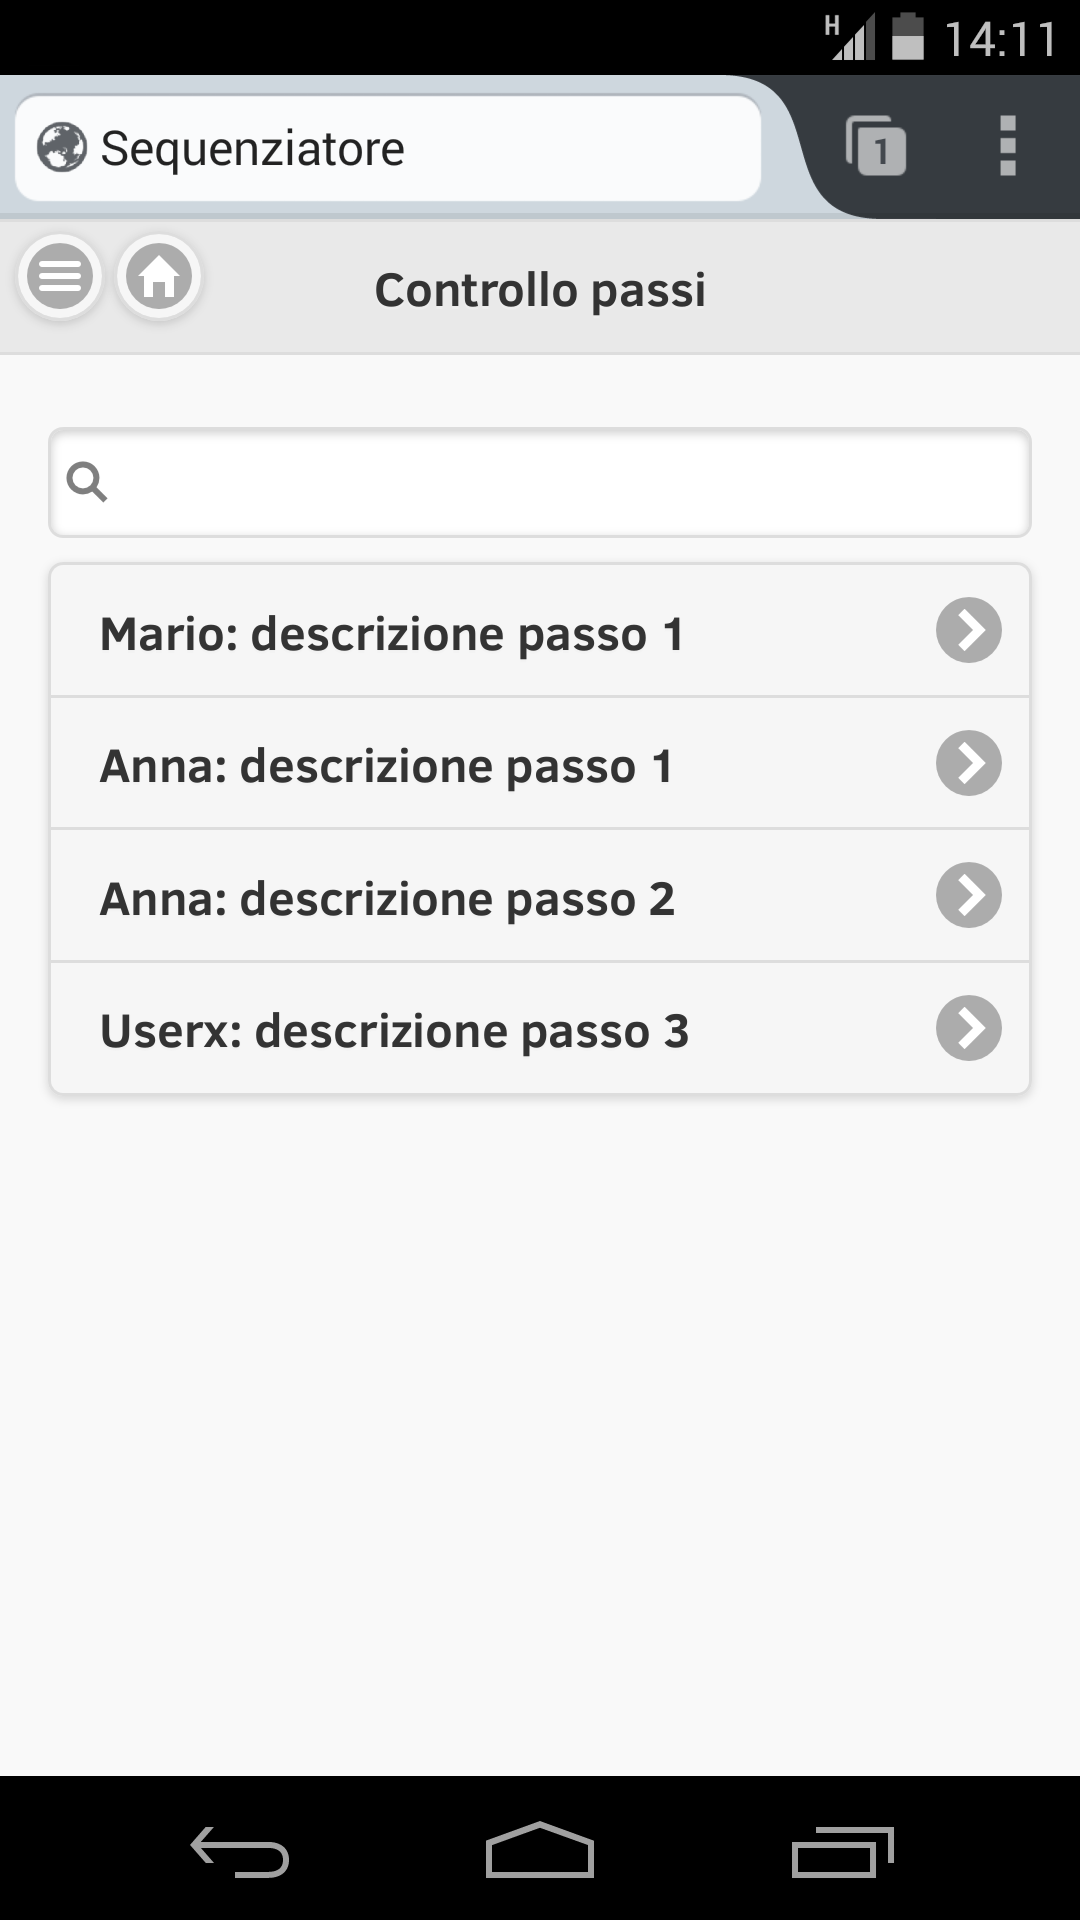
\includegraphics[width=0.5\textwidth]
{./screen/CheckStep.png}} \caption{Scelta di un passo che richiede approvazione}
\label{fig:Fcheckstep}
\end{figure}

In questa pagina è possibile selezionare uno tra i passi in elenco. È inoltre disponibile la funzionalità di ricerca: inserendo del testo nella barra di ricerca, l'elenco si aggiornerà, con i soli passi che contengono nella descrizione o nell'username dell'utente che ha inviato i dati, il testo oggetto della ricerca.
Per ripristinare l'elenco è sufficiente cancellare il testo nella barra dell'elenco.

In altro a sinistra sono presenti i seguenti pulsanti:
\begin{itemize}
\item \textbf{Home:} pulsante che consente di tornare alla \hyperref[home]{pagina principale};
\item \textbf{Opzioni:} apre il pannello laterale in cui è consentita la \hyperref[logout]{chiusura della sessione}.
\end{itemize}

\paragraph*{Possibili errori:}
\begin{itemize}
\item \hyperref[e1]{E1}: \textit{javascript\ped{G}} disabilitato;
\item \hyperref[e3]{E3}: errore di connessione al \textit{server\ped{G}}.
\end{itemize}

\subsubsection{Approvazione di un passo}

In figura \hyperref[fig:Fapprove]{figura \ref{fig:Fapprove}}, è rappresentata la schermata di visualizzazione dei dati di un passo che richiede approvazione, accessibile dopo aver effettuato l'autenticazione.

\begin{figure}[H] \centering 
\frame{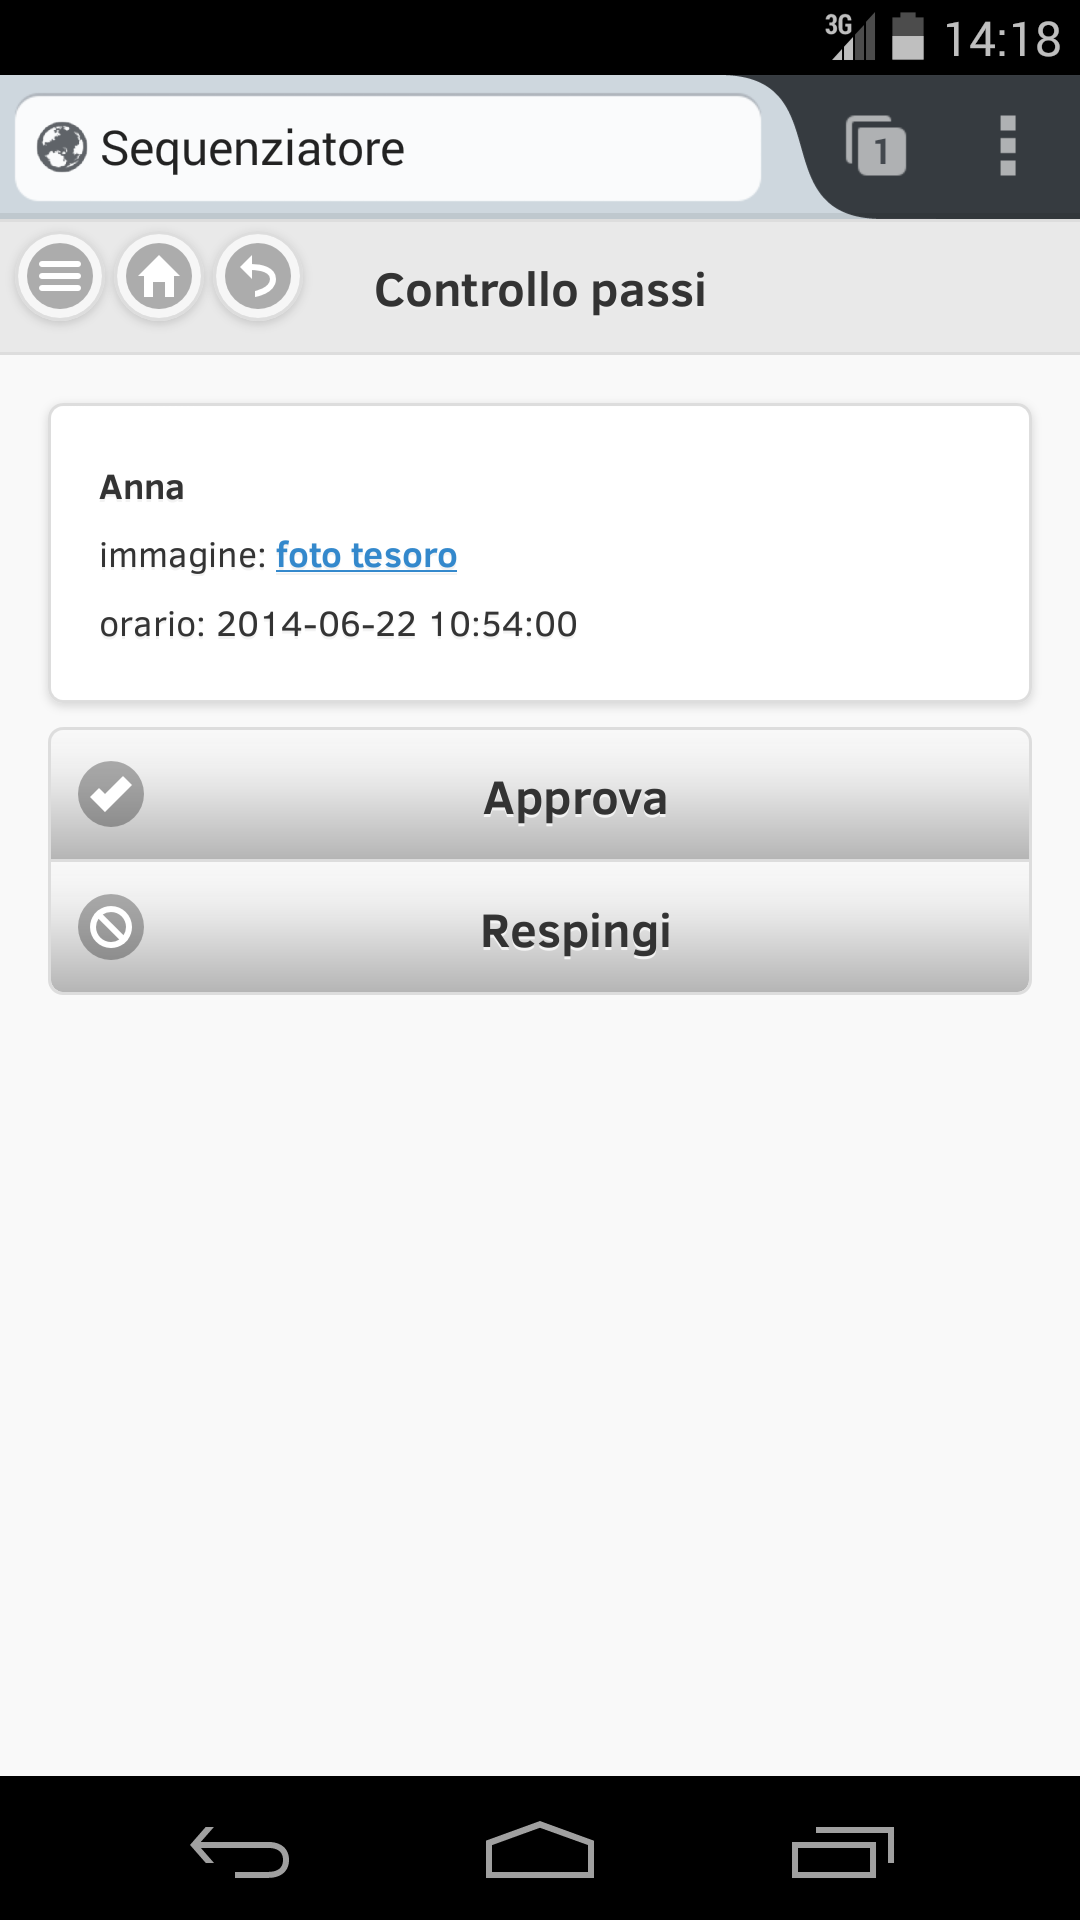
\includegraphics[width=0.5\textwidth]
{./screen/Approve.png}} \caption{Visualizzazione dei dati di un passo}
\label{fig:Fapprove}
\end{figure}

Questa pagina contiene l'elenco dei dati da un utente riguardanti il passo selezionato. 
Premendo il pulsante ``Approva'' è possibile approvare il passo selezionato, mentre, premendo il pulsante ``respingi'' il passo verrà respinto. In entrami i casi, l'esito viene inviato all'utente interessato.

In altro a sinistra sono presenti i seguenti pulsanti:
\begin{itemize}
\item \textbf{Home:} pulsante che consente di tornare alla \hyperref[home]{pagina principale};
\item \textbf{Opzioni:} apre il pannello laterale in cui è consentita la \hyperref[logout]{chiusura della sessione};
\item \textbf{Indietro:} pulsante che consente di tornare alla scelta di un passo in attesa di approvazione.
\end{itemize}

\paragraph*{Possibili errori:}
\begin{itemize}
\item \hyperref[e1]{E1}: \textit{javascript\ped{G}} disabilitato;
\item \hyperref[e3]{E3}: errore di connessione al \textit{server\ped{G}}.
\end{itemize}


\subsection{Gestione di un processo}
\label{gestione}

\subsubsection{Scelta di un processo}

In figura \hyperref[fig:Fprocesses]{figura \ref{fig:Fprocesses}}, è rappresentata la schermata di gestione dei processi, accessibile dopo aver effettuato l'autenticazione, che consente di selezionare un processo per gestirlo.

\begin{figure}[H] \centering 
\frame{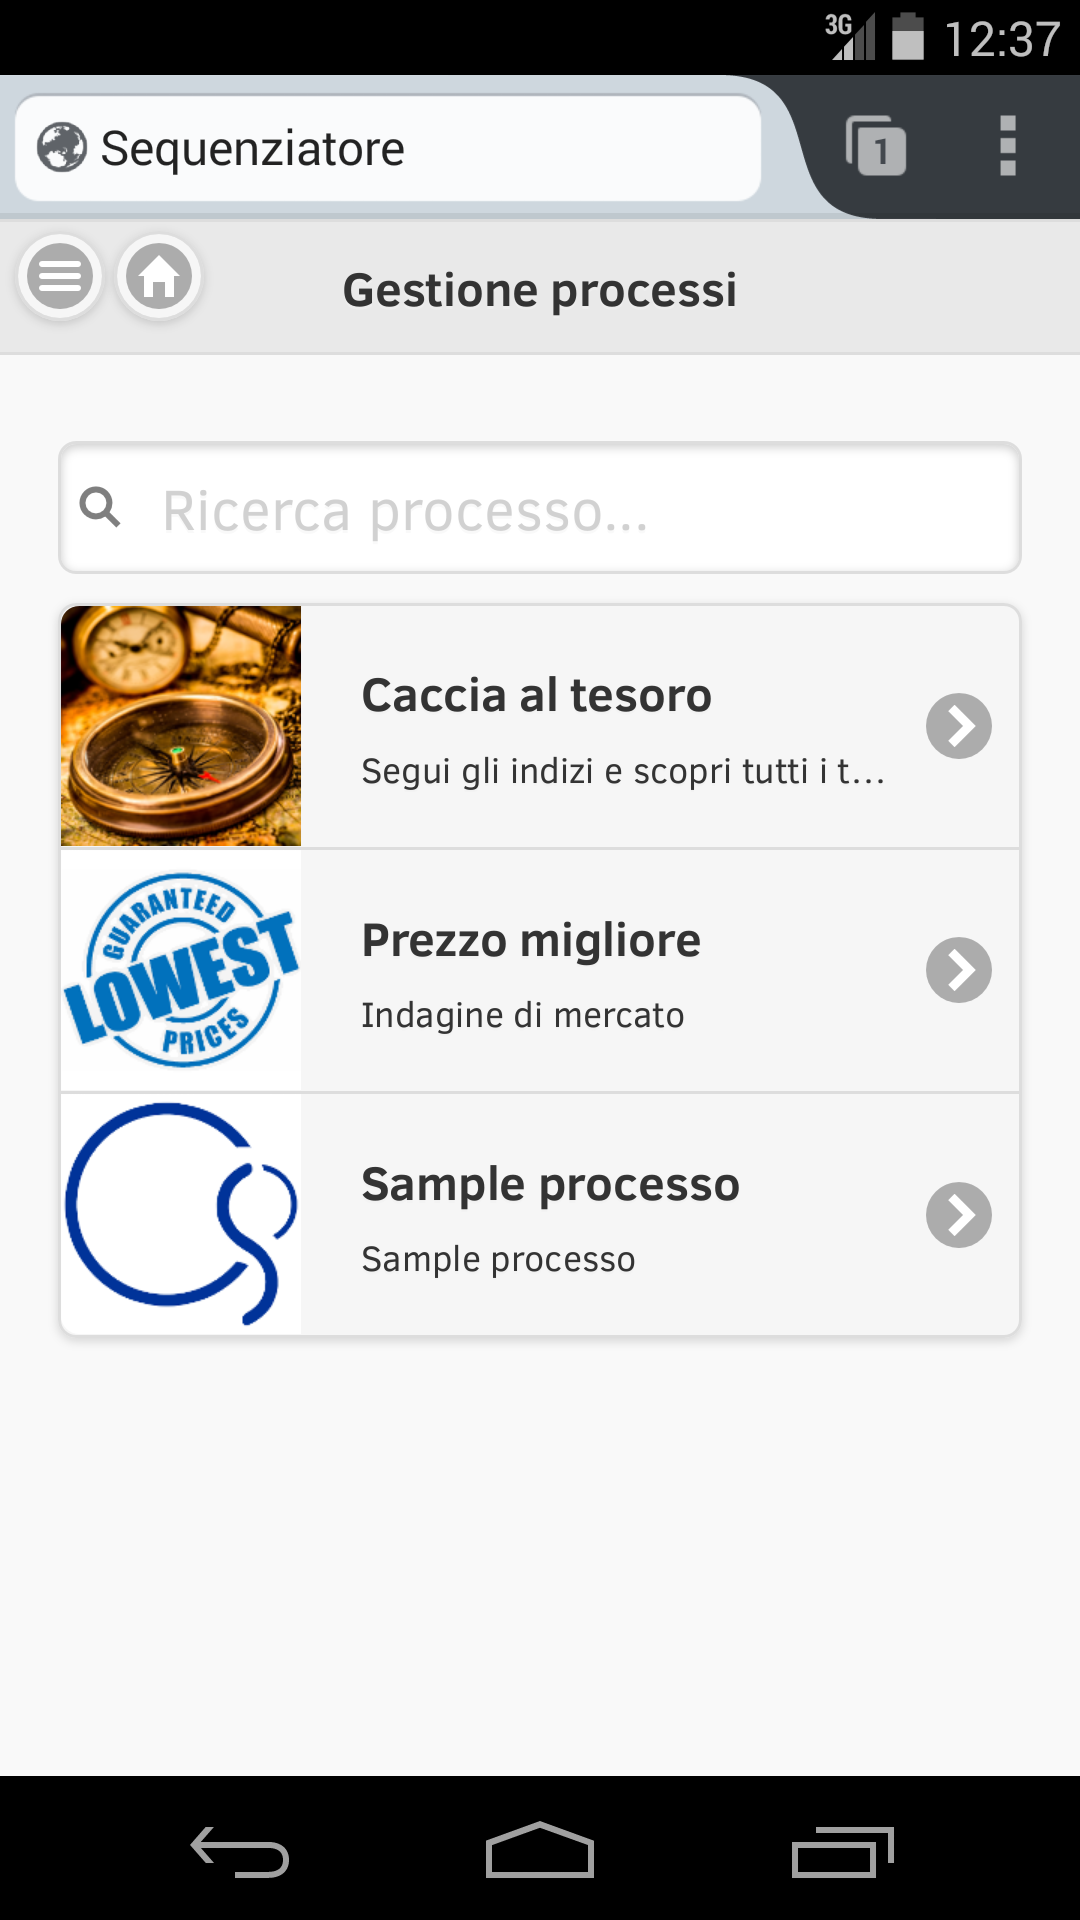
\includegraphics[width=0.5\textwidth]
{./screen/Processes.png}} \caption{Scelta processo}
\label{fig:Fprocesses}
\end{figure}

In questa pagina è possibile selezionare uno tra i processi in elenco. È inoltre disponibile la funzionalità di ricerca: inserendo del testo nella barra di ricerca (con suscritto ``Ricerca processo''), l'elenco si aggiornerà, con i soli processi che contengono nel titolo o nella descrizione, il testo oggetto della ricerca.
Per ripristinare l'elenco è sufficiente cancellare il testo nella barra dell'elenco, o premere il pulsante a forma di ``x''.

In altro a sinistra sono presenti i seguenti pulsanti:
\begin{itemize}
\item \textbf{Home:} pulsante che consente di tornare alla \hyperref[home]{pagina principale};
\item \textbf{Opzioni:} apre il pannello laterale in cui è consentita la \hyperref[logout]{chiusura della sessione}.
\end{itemize}

\paragraph*{Possibili errori:}
\begin{itemize}
\item \hyperref[e1]{E1}: \textit{javascript\ped{G}} disabilitato;
\item \hyperref[e3]{E3}: errore di connessione al \textit{server\ped{G}}.
\end{itemize}

\subsubsection{Scelta di un passo del processo}

In figura \hyperref[fig:Fprocess]{figura \ref{fig:Fprocess}}, è rappresentata la schermata di gestione di un processo, accessibile dopo aver effettuato l'autenticazione, che consente di selezionare un passo del processo in gestione.

\begin{figure}[H] \centering 
\frame{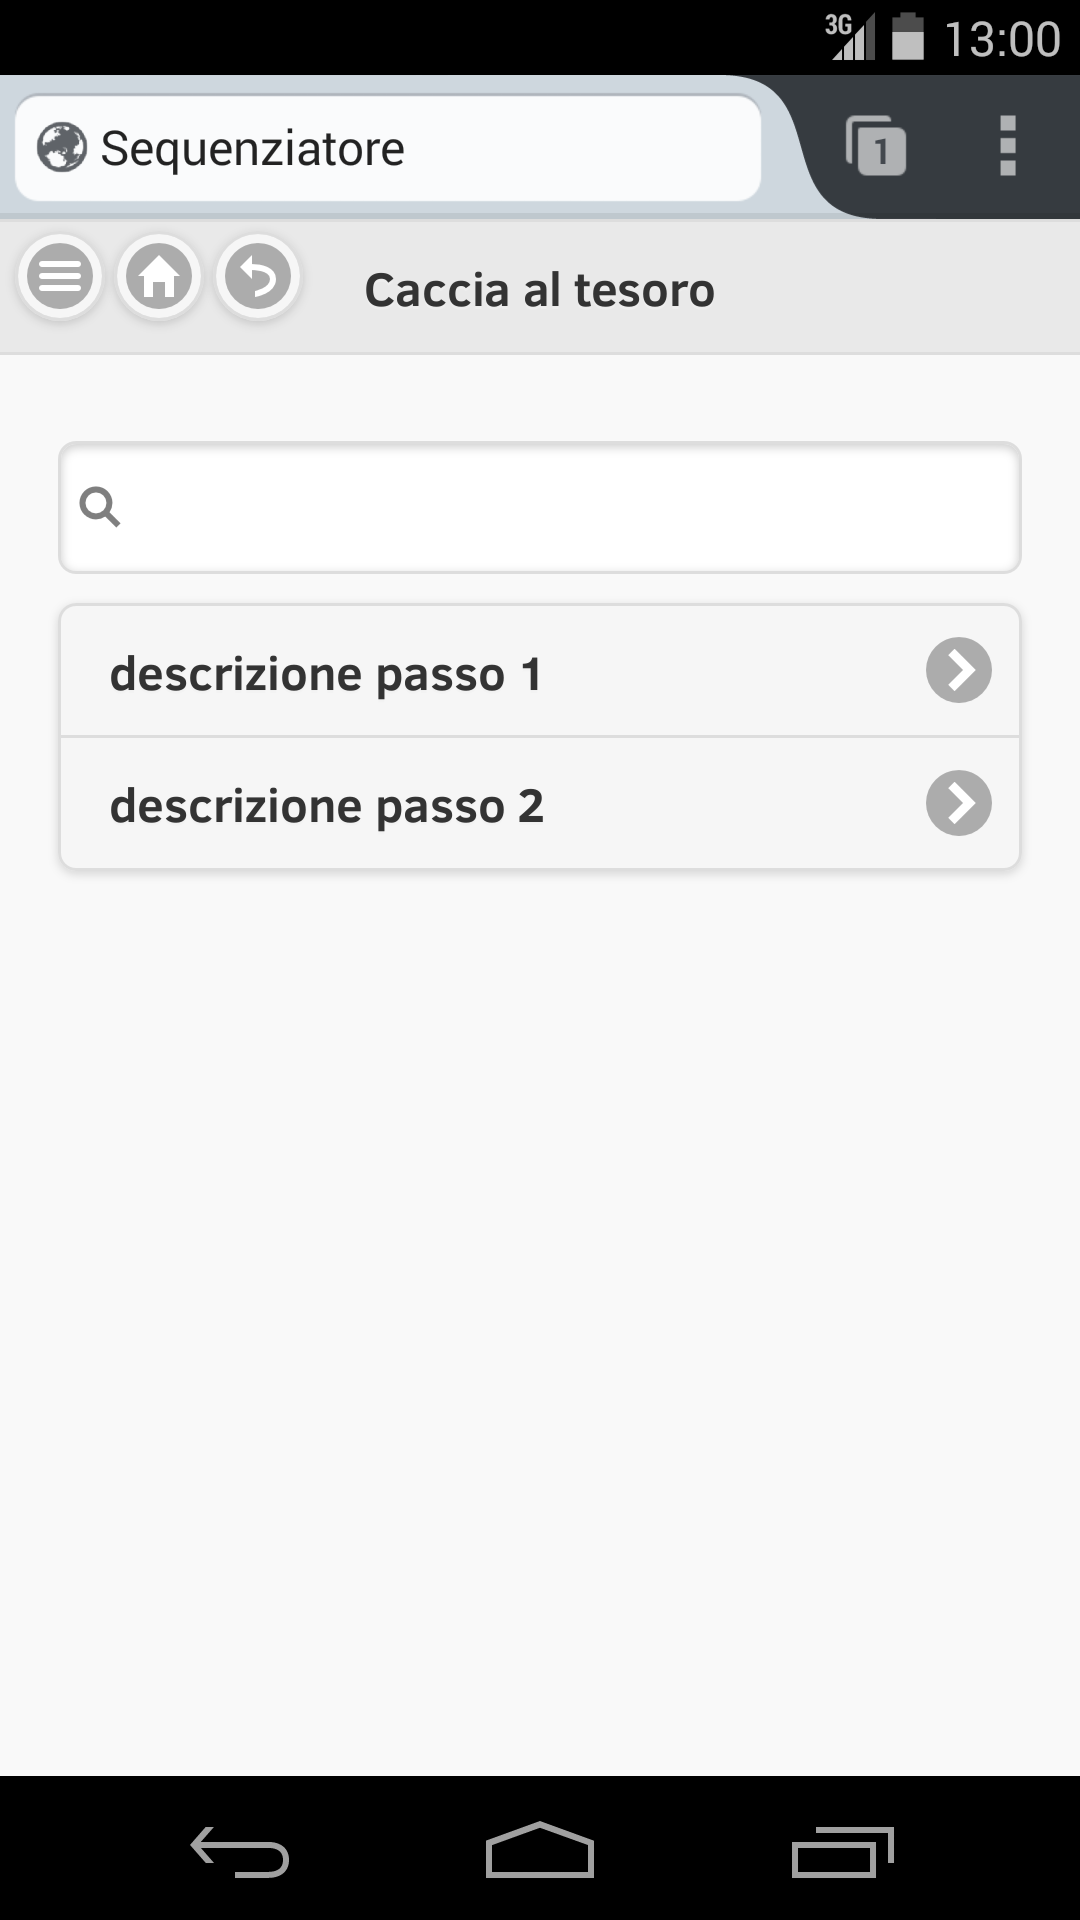
\includegraphics[width=0.5\textwidth]
{./screen/Process.png}} \caption{Scelta di un passo}
\label{fig:Fprocess}
\end{figure}

In questa pagina è possibile selezionare uno tra i passi in elenco. È inoltre disponibile la funzionalità di ricerca: inserendo del testo nella barra di ricerca, l'elenco si aggiornerà, con i soli passi che contengono nella descrizione, il testo oggetto della ricerca.
Per ripristinare l'elenco è sufficiente cancellare il testo nella barra dell'elenco.

In altro a sinistra sono presenti i seguenti pulsanti:
\begin{itemize}
\item \textbf{Home:} pulsante che consente di tornare alla \hyperref[home]{pagina principale};
\item \textbf{Opzioni:} apre il pannello laterale in cui è consentita la \hyperref[logout]{chiusura della sessione};
\item \textbf{Indietro:} pulsante che consente di tornare alla scelta di un processo.
\end{itemize}

\paragraph*{Possibili errori:}
\begin{itemize}
\item \hyperref[e1]{E1}: \textit{javascript\ped{G}} disabilitato;
\item \hyperref[e3]{E3}: errore di connessione al \textit{server\ped{G}}.
\end{itemize}

\subsubsection{Visualizzazione dei dati di un passo}

In figura \hyperref[fig:Fstepdata]{figura \ref{fig:Fstepdata}}, è rappresentata la schermata di visualizzazione dei dati di un passo, accessibile dopo aver effettuato l'autenticazione.

\begin{figure}[H] \centering 
\frame{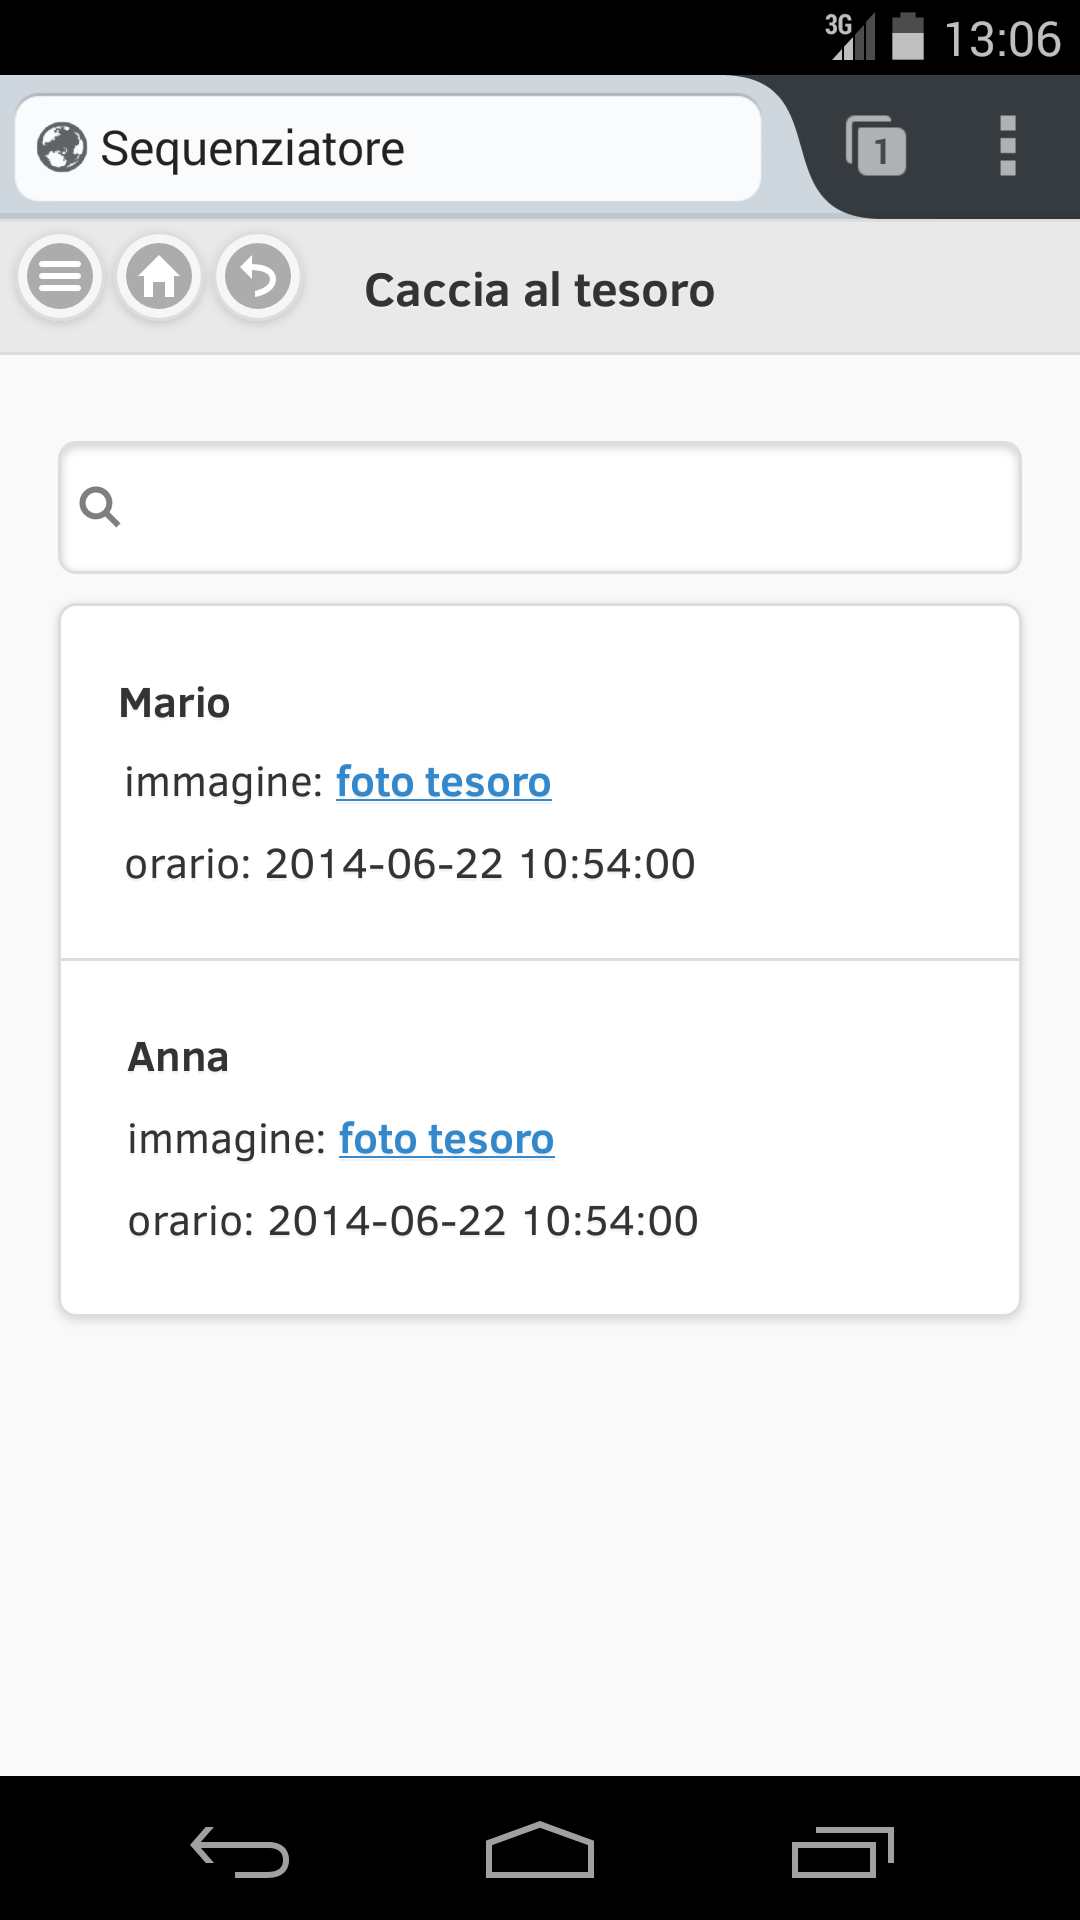
\includegraphics[width=0.5\textwidth]
{./screen/StepData.png}} \caption{Visualizzazione dei dati di un passo}
\label{fig:Fstepdata}
\end{figure}

Questa pagina è composta dall'elenco dei dati inviati dagli utenti riguardanti il passo selezionato. 
È disponibile la funzionalità di ricerca: inserendo del testo nella barra di ricerca, l'elenco si aggiornerà, con i soli dati che contengono nella descrizione, il testo oggetto della ricerca.
Per ripristinare l'elenco è sufficiente cancellare il testo nella barra dell'elenco.

In altro a sinistra sono presenti i seguenti pulsanti:
\begin{itemize}
\item \textbf{Home:} pulsante che consente di tornare alla \hyperref[home]{pagina principale};
\item \textbf{Opzioni:} apre il pannello laterale in cui è consentita la \hyperref[logout]{chiusura della sessione};
\item \textbf{Indietro:} pulsante che consente di tornare alla scelta di un passo del processo in gestione.
\end{itemize}

\paragraph*{Possibili errori:}
\begin{itemize}
\item \hyperref[e1]{E1}: \textit{javascript\ped{G}} disabilitato;
\item \hyperref[e3]{E3}: errore di connessione al \textit{server\ped{G}}.
\end{itemize}

\subsection{Chiusura della sessione}
\label{logout}
In figura \hyperref[fig:Flogout]{figura \ref{fig:Flogout}}, è rappresentato il pannello laterale, visualizzabile premendo il pulsante opzioni (vedi pulsante in alto a sinistra in \hyperref[fig:Fhome]{figura \ref{fig:Fhome}}), da qualsiasi pagina accessibile dopo aver effettuato l'autenticazione.

\begin{figure}[H] \centering 
\frame{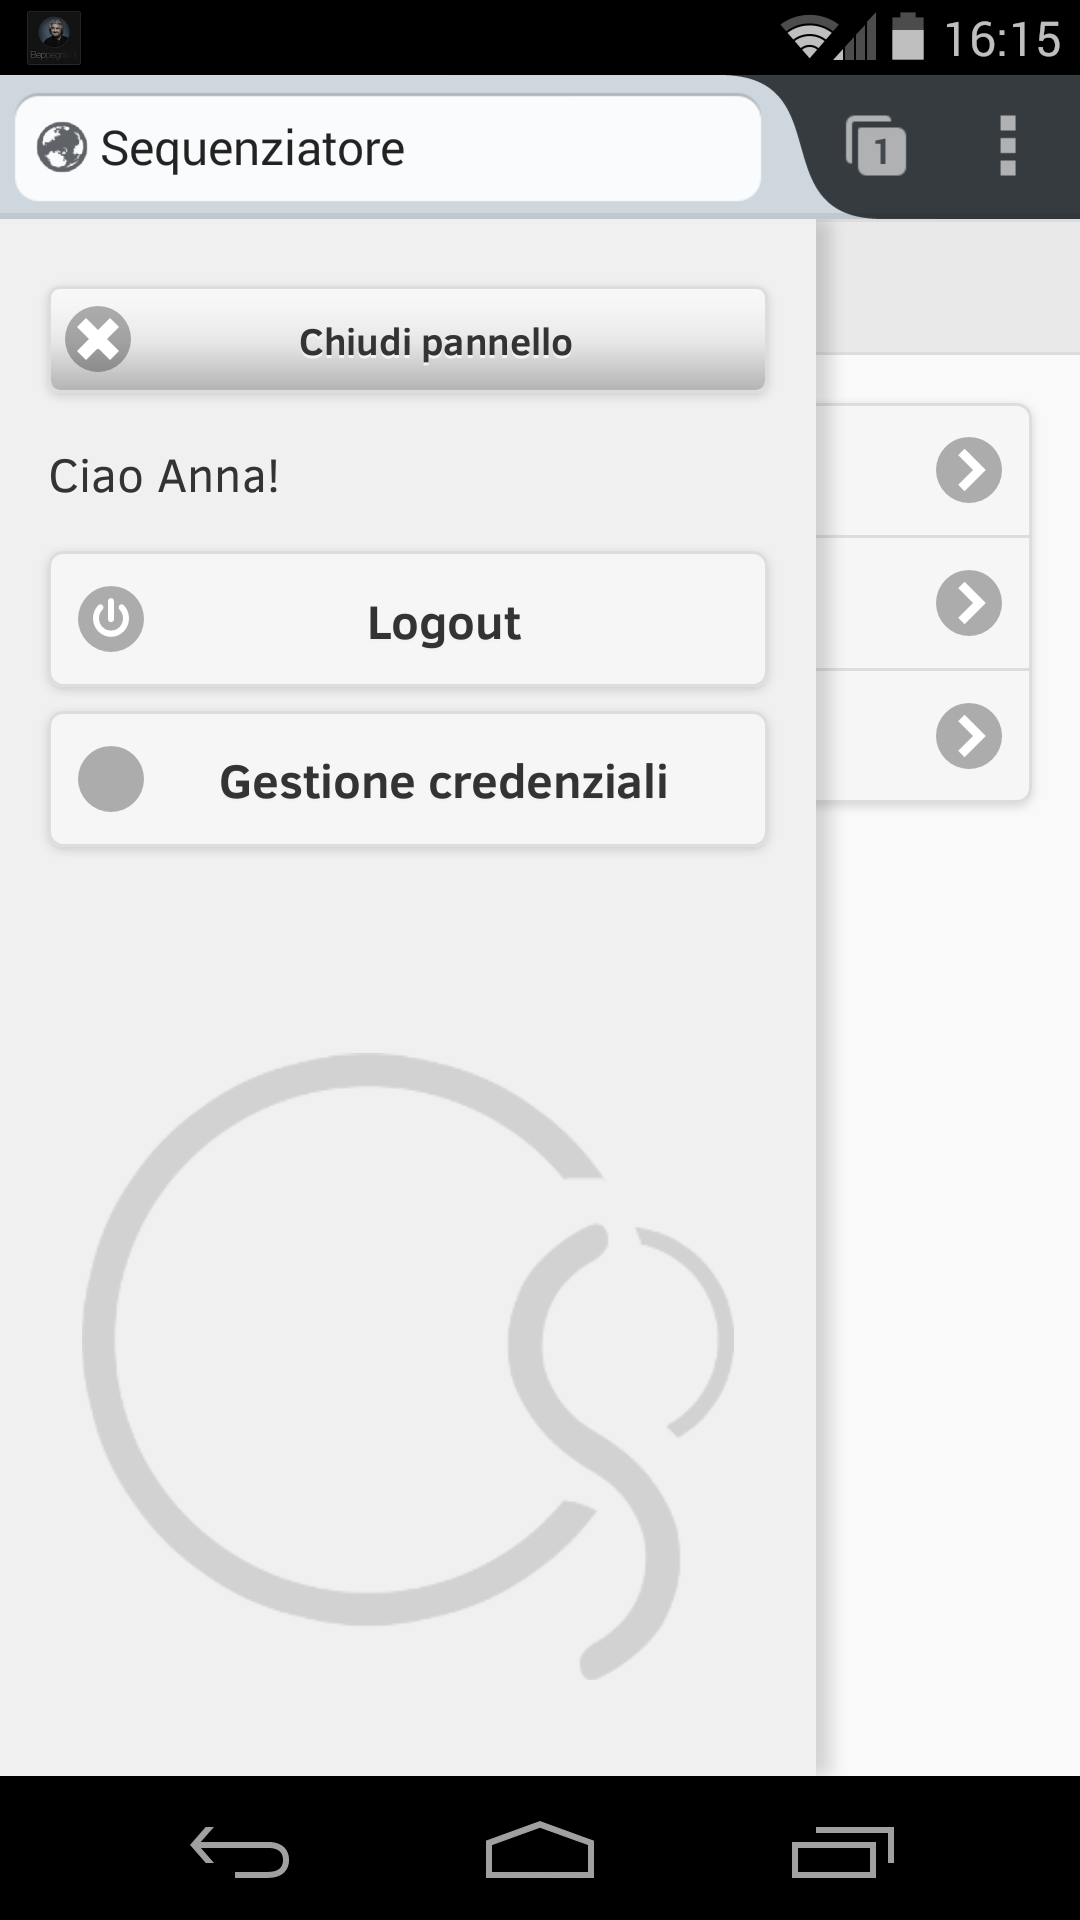
\includegraphics[width=0.5\textwidth]
{./screen/Logout.png}} \caption{Pannello laterale}
\label{fig:Flogout}
\end{figure}

Premendo il pulsante ``chiudi pannello'' è possibile ritornare alla pagina da cui il pannello è stato aperto.
Premendo il pulsante ``Logout'' l'utente ritornerà alla pagina di \hyperref[autenticazione]{autenticazione}, e i suoi dati di sessione\ped{G} vengono eliminati.

\subsubsection*{Possibili errori:}
\begin{itemize}
\item \hyperref[e1]{E1}: \textit{javascript\ped{G}} disabilitato.
\end{itemize}

\appendix
\section{Descrizione messaggi di errore}
\label{errori}
\section{Glossario}
\label{glossario}

Sono qui di seguito elencate in ordine alfabetico, le definizioni di tutti i termini contrassegnati con il pedice "G" nel documento.

\subsection*{"A"}
\addcontentsline{toc}{subsection}{\protect\numberline{}A}
\begin{itemize}
\item \textbf{Android}:\\ sistema operativo open source\ped{G} per dispositivi mobili sviluppato da Google Inc.
\end{itemize}
\subsection*{"B"}
\begin{itemize}
\item \textbf{Browser}:\\ programma utilizzato per la navigazione dei contenuti presenti nel World Wide Web;
tecnicamente, un browser e un’applicazione client\ped{G} che utilizza il protocollo HTTP\ped{g} per inoltrare le richieste dell’utente ad un web server\ped{G}.
\end{itemize}

\subsection*{"C"}
\addcontentsline{toc}{subsection}{\protect\numberline{}C}
\begin{itemize}
\item \textbf{Chrome}:\\ browser\ped{G} proprietario sviluppato da Google, basato su un progetto opensource\ped{G};
\item \textbf{Chrome for iOS\ped{G}}:\\ versione per iOS\ped{G} di Chrome\ped{G};
\item \textbf{Chromium}:\\ browser\ped{G} opensource, è il core di Chrome\ped{G};
\item \textbf{Client}:\\ computer o programma che inoltra le richieste dell’utente ad un programma server\ped{G}.
\end{itemize}

\subsection*{"D"}
\addcontentsline{toc}{subsection}{\protect\numberline{}D}
\begin{itemize}
\item \textbf{Dati di sessione}:\\ Dati salvati nel dispositivo dell'utente, che associano l'utente ad una applicazione. Nel progetto \progetto{}, tali dati consentono al programma di conoscere se l'utente è autenticato, o se deve effettuare il \textit{login}.
\end{itemize}

\subsection*{"H"}
\addcontentsline{toc}{subsection}{\protect\numberline{}H}
\begin{itemize}
\item \textbf{HTML}:\\ linguaggio di markup\ped{G} per la strutturazione delle pagine web.
\end{itemize}

\subsection*{"I"}
\addcontentsline{toc}{subsection}{\protect\numberline{}I}
\begin{itemize}
\item \textbf{iOS}:\\ sistema operativo\ped{G} sviluppato da Apple Inc, disponibile solamente su dispositivi mobili Apple;
\item \textbf{Internet Explorer}:\\ browser\ped{G} proprietario sviluppato da Microsoft.
\end{itemize}

\subsection*{"M"}
\addcontentsline{toc}{subsection}{\protect\numberline{}M}
\begin{itemize}
\item \textbf{Markup}:\\ in generale un linguaggio di markup è un insieme di regole che descrivono i meccanismi di rappresentazione (strutturali, semantici o presentazionali) di un testo;
\item \textbf{Mozilla Firefox}:\\ browser\ped{G} opensource\ped{G} sviluppato da Mozilla Foundation.
\end{itemize}

\subsection*{"O"}
\addcontentsline{toc}{subsection}{\protect\numberline{}O}
\begin{itemize}
\item \textbf{Open source}:\\ in informatica, indica un software i cui autori (più precisamente i detentori dei diritti) ne permettono e favoriscono il libero studio e l'apporto di modifiche da parte di altri programmatori indipendenti;
\item \textbf{Opera}:\\ browser\ped{G} free sviluppato da Opera Software.
\end{itemize}

\subsection*{"P"}
\addcontentsline{toc}{subsection}{\protect\numberline{}P}
\begin{itemize}
\item \textbf{Passo}:\\ nel contesto del progetto \progetto{}, un passo è inteso come una unità di un workflow\ped{G}, e può essere visto come un insieme di dati che devono essere raccolti al fine di completarlo;
\item \textbf{PDF}:\\ formato di un file basato su un linguaggio di descrizione di pagina, utile per rappresentare documenti in modo indipendente dall'hardware e dal software utilizzati per generarli o per visualizzarli;
\item \textbf{Process owner}:\\ per process owner nel contesto del progetto si intende un utente che può creare processi a cui gli utenti base possono partecipare, e il quale ha privilegi speciali riguardo l'accesso delle informazioni inviate dagli utenti; questi privilegi sono utili a determinare la correttezza di dei data che necessitano una verifica umana.
\end{itemize}

\subsection*{"S"}
\addcontentsline{toc}{subsection}{\protect\numberline{}S}
\begin{itemize}
\item \textbf{Safari}:\\ browser\ped{G} sviluppato da Apple Inc.;
\item \textbf{Safari for iOs}:\\ versione per iOs\ped{G} di Safari;
\item \textbf{Server}:\\ componente che fornisce un qualsiasi servizio ad altre componenti denominate client\ped{G} attraverso una rete di computer o direttamente in locale;
\item \textbf{Sistema operativo}: software\ped che ha il compito di gestire e controllare tutto il traffico di dati all’interno del computer e fra questo e tutte le periferiche, operando anche come intermediario fra hardware\ped{G} e software\ped{G} di sistema ed i diversi programmi in esecuzione;
\item \textbf{Software}:\\ termine generico che definisce programmi e procedure utilizzati per far eseguire al computer un determinato compito.
\end{itemize} 

\subsection*{"U"}
\addcontentsline{toc}{subsection}{\protect\numberline{}U}
\begin{itemize}
\item \textbf{URL}:\\ sequenza di caratteri che identifica univocamente l'indirizzo di una risorsa \textit{web}.
\end{itemize}

\end{document}